
\chapter{Formalisations and proofs}\label{sec:formalisation}

\section{Logarithmic distance and proximity order \statusgreen}\label{sec:proximity}
Consider the set of bit sequences with fixed length $d$ as points in a space. We can define a distance metric $\chi$ such that
the distance between two such sequences is defined as the bigendian numerical value of their bitwise XOR ($\xor$).

\begin{definition}{XOR distance ($\chi$)}\label{def:xor}
\begin{equation}
\chi(x, y) \defeq \mathit{Uint}(x  \xor y)
\end{equation}
\end{definition}

Given the fixed length $d>0$, there is a maximum distance in this space, and thus we can define the notion of \emph{normalised distance} and its inverse, \emph{proximity}:

\begin{definition}{normalised XOR distance ($\overline{\chi}$)}\label{def:normalisedxor}
\begin{equation}
\overline{\chi}(x, y) \defeq \frac{\chi(x,y)}{2^d-1}
\end{equation}
\end{definition}

\begin{definition}{proximity}\label{def:proximity}
\begin{equation}
\mathit{Proximity}(x, y) \defeq \frac{1}{\overline{\chi}(x,y)}
\end{equation}{}
\end{definition}


\emph{Proximity order (PO)} is a discrete logarithmic scaling of proximity.


\begin{definition}{Proximity order ($\PO$)}\label{def:xorPO}
\begin{equation}
\begin{split}
\PO&: \Keys \times\Keys\mapsto \overline{0,d}\\
\PO(x,y) &\defeq 
\begin{cases}
d & \text{ if } x=y\\
\mathit{int}(\log_2(\mathit{Proximity}(x, y)))&\text{otherwise}\\
\end{cases}
\end{split}
\end{equation}
\end{definition}


In practice, $\PO(x,y)$ is the length of the longest common prefix in the bigendian binary representation of $x$ and $y$. So in practice it is calculated by counting the matching bits from the left. The maximum value of proximity is the number of bits $d$. Kademlia falls in the prefix matching class of DHT-s \cite{rowstron2001pastry,zhao2004tapestry}.

Taking the proximity order relative to a fixed point $x_0$ partitions the points in
the space (of bit sequences of length $d$) into equivalence classes. Points in each class are at
most half as distant from $x_0$ as items in the previous class. Furthermore, any two points belonging to the same class are at most half as distant from each other as they are from $x_0$. We can generalise the important properties of the proximity order function as follows:

\begin{definition}{Proximity order definitional properties}\label{def:PO}
\begin{equation}
\PO: \Keys\times \Keys\mapsto \overline{0,d}
\end{equation}

% \begin{equation}
\begin{subequations}
  \begin{align}
    \label{eq:PO-constraint-symmetry} \text{reflexivity:  }&\forall x,y\in \mathcal{K}, \PO(x,y)=\PO(y,x)\\
    \label{eq:PO-constraint-monotonicity}\text{monotonicity:   }&\forall x,y,z\in \mathcal{K}, \PO(x,y)=k \land  \PO(x,z)=k \Rightarrow  \PO(y,z)>k\\
\label{eq:PO-constraint-transitivity}\text{transitivity:   }&\forall x,y,z\in \mathcal{K}, \PO(x,y)<\PO(y,z) \Rightarrow \PO(x,z)=\PO(x,y)
   \end{align}
\end{subequations}
% \end{equation}
\end{definition}

Given a set of points uniformly distributed in the space (e.g., the results of a hash function), proximity orders map onto a series of subsets with cardinalities on a negative exponential scale, i.e., PO bin 0 has half of the points of any random sample, PO bin 1 has one fourth, PO bin 2 one eighth, etc.

\section{Proximity orders in graph topology \statusgreen}

This section gives a graph theoretical  approach to Kademlia topology \cite{aspnes2007skip}.
Consider a set of points $V$ in the space with a logarithmic distance and 
a binary relation $R$. Define a directed graph where every point in the set is a vertex and any two vertices $x$ and $y$ are  connected with an edge if they are in relation $R$. 


Points that are in relation $R$ with a particular point $x_0$ can be indexed by their proximity order relative to $x_0$. This index is called \gloss{Kademlia table}.
The Kademlia table can serve as the basis for local decisions in graph traversal where the task is to find a path between two points. 


\begin{definition}{Kademlia table}\label{def:kademlia-table}
\begin{equation}
\begin{split}
&\mathit{Kad}_x: \overline{0,d} \mapsto \mathcal{P}(\mathit{V})\\
&\forall y, \langle x, y \rangle \in \mathit{Edges}(G) \rightarrow y \in \mathit{Kad}_x(p) \Longleftrightarrow \PO(x,y)=p 
\end{split}
\end{equation}
\end{definition}

We say that a point has \emph{kademlia connectivity} (or the point's connectivity has  the kademlia property) if (1) it is connected to at least one node for each proximity order up to (but excluding) some maximum value $d$ (called the \gloss{saturation depth}) and (2) it is connected to all nodes whose proximity order relative to the node is greater or equal to $d$.

\begin{definition}{Kademlia connectivity}\label{sec:kademlia-connectivity}
\begin{equation}
\exists d, 0\leq d \leq l, \text{such that}
\begin{subequations}
(1)\forall p<d, |\mathit{Kad}_x(p)|>0 \\
(2)\forall y\in V, PO(x,y)=p\geq d \longrightarrow y\in\mathit{Kad}_x(p) 
\end{subequations}
\end{equation}
\end{definition}


If each point of a connected subgraph has kademlia connectivity, then we say the subgraph has a \gloss{Kademlia topology}. In a graph with kademlia topology, (1) a path between any two points exists, (2) it can be found using only local decisions on each hop and (3) is guaranteed to terminate in no more steps than the depth of the destination plus one. 

The procedure is as follows. Given point $x$ and $y$, construct the path $x_0=x , x_1, ..., x_k=y$ such that $x_{i+1}\in \mathit{PO}(x_i, x_{i+1})=\mathit{PO}(x_i, y)$, i.e., starting from the source point, choose the next point from the PO bin that the destination address falls into: because of the assumption of kademlia connectivity (1) such a point exists. Due to our previous conjecture, the actual bin is monotonically increasing at each step and can start with zero, therefore for every $0<i<=l$, $\mathit{PO}(x_{i}, y)\geq i$. So there exists a $d\leq d_y$, such that 
$\mathit{PO}(x_{d}, y)\geq d_y$, which together with kademlia connectivity criterion (2) entails that either $x_d=y$ and $k=d$, or $y$ is connected to $x_d$, so we can choose $x_{d+1}=y$, and $k=d+1\leq d_y+1$.

\begin{theorem}{In graphs with kademlia topology, any two points are connected and traversal path can be constructed based on local kademlia tables where the path length upper bound is logarithmic in the number of nodes.}

\begin{proof}



\qed
\end{proof}
\end{theorem}

\section{Constructing kademlia topology \statusred}

\section{Complexity of filling up a postage stamp batch \statusgreen}\label{sec:complexity-filling}

A postage batch is utilised optimally if each of its collision slots are filled. Although hashes are uniform, due to variance one cannot guarantee that $2^d$ independent hashes map to the collision slots of a batch of depth $d$.
We presented various ways of mining chunks: by (1) choosing the nonce of a trojan chunk (see \ref{sec:trojan}), (2) choosing the encryption key (see \ref{sec:postage-stamps}), or choosing the index of a single owner chunk (see \ref{sec:addressed-envelopes}). Whichever way we are mining the chunks, the chance of finding an address that takes the $i$-th collision slot of the stamp, i.e., 


\begin{equation}
\mathit{PO}(\mathit{H}(\mathit{Enc}(k, c)), \mathit{CS}(i))\geq\mathit{D},
\text{ where }\mathit{CS}(i)\defeq i*2^{256-D}
\text{ for }0\leq i\leq  2^D.
\end{equation}

Now, if the user wishes to always fill their postage stamp batch before using another one, for each new chunk there is one less choice to pick a free collision slot. Let the probabilistic variable $X^n_i$ denote  the number of trials one needed to find a slot when $i$ out of $n$ slots are free. The probability that it is at least 1 is $\frac{n-i}{n}$, and in general:


\begin{equation}\label{eq:conditional}
\mathit{P}(X^n_i\geq j+1|X^n_i\geq j)=\frac{n-i}{n}\\
\end{equation}

The expected number of trials for the $i$-th chunk is 

 \begin{subequations}   \begin{align}
\mathit{E}(X^n_i)&=\sum^\infty_{j=1}j\mathit{P}(X^n_i=j)\\
&=\mathit{P}(X^n_i\geq 1)-\mathit{P}(X^n_i\geq 2)+2(\mathit{P}(X^n_i\geq 2)-P(X^n_i\geq 3))+\ldots\\
&= \mathit{P}(X^n_i\geq 1)+\mathit{P}(X^n_i\geq 2)+\ldots
\end{align} \end{subequations}

Multiplying both sides with $\frac{n-i}{n}$, then using  the equivalence in  \ref{eq:conditional}:

 \begin{subequations}   \begin{align}
\mathit{E}(X^n_i)\frac{n-i}{n}&=\mathit{P}(X^n_i\geq 1)\mathit{P}(X^n_i\geq 2|X^n_i\geq 1)+\mathit{P}(X^n_i\geq 2)\mathit{P}(X^n_i\geq 3|X^n_i\geq 2)+\ldots\\
&=\mathit{P}(X^n_i\geq 2)+\mathit{P}(X^n_i\geq 3)+\ldots\\
&=\mathit{E}(X^n_i)-\mathit{P}(X^n_i\geq 1)\\
&=\mathit{E}(X^n_i)-\frac{n-i}{n}
\end{align} \end{subequations}

From this, we solve to $\mathit{E}(X^n_i)$:

 \begin{subequations}   \begin{align}
\mathit{E}(X^n_i)(1-\frac{n-i}{n})&=1\\
\mathit{E}(X^n_i)&=\frac{n}{i}
\end{align} \end{subequations}

Averaging for the whole batch ($n=2^D$) gives%
%
\footnote{see harmonic series 
\url{https://en.wikipedia.org/wiki/Harmonic\_series\_(mathematics)\#Rate\_of\_divergence}.}

 \begin{subequations}   \begin{align}
\sum_{i=1}^{2^D}\frac{2^D}{i}\frac{1}{2^D}
&=\sum_{i=1}^{2^D}\frac{1}{i}\\
&=\mathit{ln}(2^D)+1\\
&=\frac{\mathit{log}_2(2^D)}{\mathit{log}_2(e)}+1\\
&=D*0.6931+1
\end{align} \end{subequations}

\section{Average hop count for chunk retrieval  \statusred}

This section gives a formal estimation of the expected hop count for a random non-cached chunk.  
Hop-count in traditional kademlia has already been  analysed \cite{roos2013comprehending, roos2015determining}.

\section{Distribution of requests \statusred}

In this section we derive the distribution of requests per PO bin that an average node experiences.

\section{epoch-based feeds \statusgreen}\label{sec:epoch-based-feeds-appendix}
\subsection{Update example \statusgreen}
 
Let's say that we want to update our resource 5 minutes later. The Unix Time is now $1534093015$.
We calculate $\mathit{epochBaseTime}(1534093015, 25) = 1509949440$.
This results in the same epoch as before $\langle  1534093015, 25\rangle$. Therefore, we decrease the level and calculate again:
$\mathit{epochBaseTime}(1534093015, 24) = 1526726656$. Thus, the next update will be located at $\langle  1526726656, 24\rangle$

If the publisher keeps updating the resource exactly every 5 minutes, the epoch grid will look like this:

{\small
\begin{tabular}{c|c}
\begin{tabular}{r|l|l}
update & timestamp & epoch representation\\
1 & 1534092715 & $\langle  1509949440, 25\rangle$\\
2 & 1534093015 & $\langle  1526726656, 24\rangle$\\
3 & 1534093315 & $\langle  1526726656, 23\rangle$\\
4 & 1534093615 & $\langle  1530920960, 22\rangle$\\
5 & 1534093915 & $\langle  1533018112, 21\rangle$\\
6 & 1534094215 & $\langle  1534066688, 20\rangle$\\
7 & 1534094515 & $\langle  1534066688, 19\rangle$\\
8 & 1534094815 & $\langle  1534066688, 18\rangle$\\
9 & 1534095115 & $\langle  1534066688, 17\rangle$\\
10 & 1534095415 & $\langle 1534066688, 16\rangle$\\
11 & 1534095715 & $\langle 1534066688, 15\rangle$\\
12 & 1534096015 & $\langle 1534083072, 14\rangle$\\
13 & 1534096315 & $\langle 1534091264, 13\rangle$\\
14 & 1534096615 & $\langle 1534095360, 12\rangle$\\
15 & 1534096915 & $\langle 1534095360, 11\rangle$
\end{tabular}
&
\begin{tabular}{r|l|l}
update & timestamp & epoch representation\\
16 & 1534097215 & $\langle 1534096384, 10\rangle$\\
17 & 1534097515 & $\langle 1534096896, 9\rangle$\\
18 & 1534097815 & $\langle 1534097408, 11\rangle$\\
19 & 1534098115 & $\langle 1534097408, 10\rangle$\\
20 & 1534098415 & $\langle 1534097920, 9\rangle$\\
21 & 1534098715 & $\langle 1534098176, 8\rangle$\\
22 & 1534099015 & $\langle 1534098432, 10\rangle$\\
23 & 1534099315 & $\langle 1534098944, 9\rangle$\\
24 & 1534099615 & $\langle 1534099200, 8\rangle$\\
25 & 1534099915 & $\langle 1534099456, 15\rangle$\\
26 & 1534100215 & $\langle 1534099456, 14\rangle$\\
27 & 1534100515 & $\langle 1534099456, 13\rangle$\\
28 & 1534100815 & $\langle 1534099456, 12\rangle$\\
29 & 1534101115 & $\langle 1534099456, 11\rangle$\\
30 & 1534101415 & $\langle 1534100480, 10\rangle$
\end{tabular}
\end{tabular}
}


\begin{figure}[htbp]
\centering
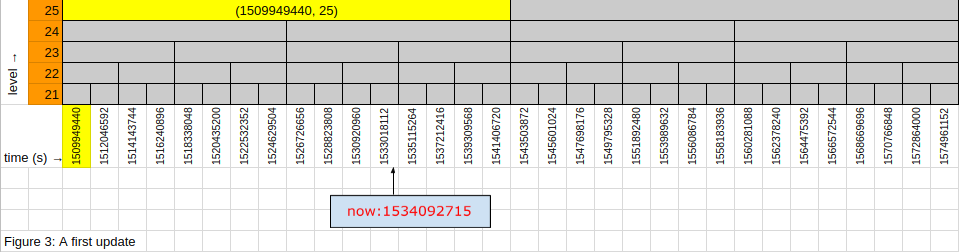
\includegraphics[width=\textwidth]{fig/feeds/00.png}\\
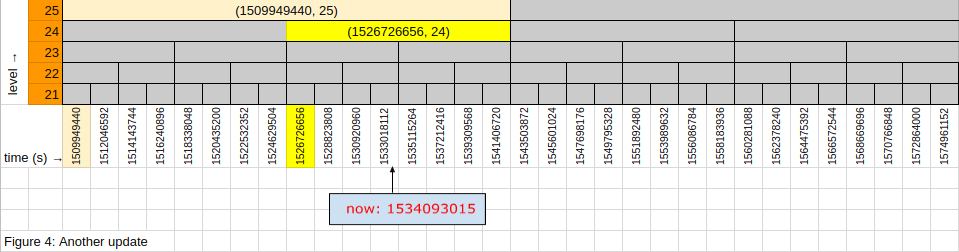
\includegraphics[width=\textwidth]{fig/feeds/01.png}\\
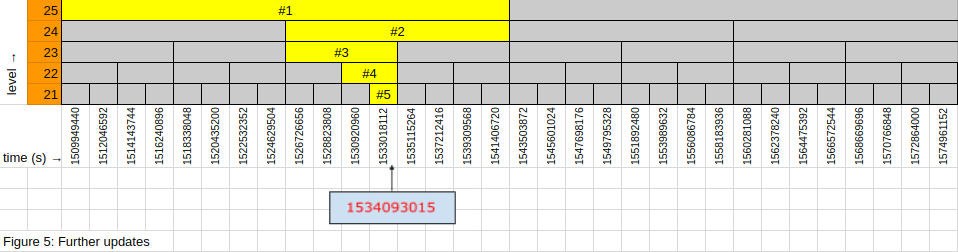
\includegraphics[width=\textwidth]{fig/feeds/02.png}\\
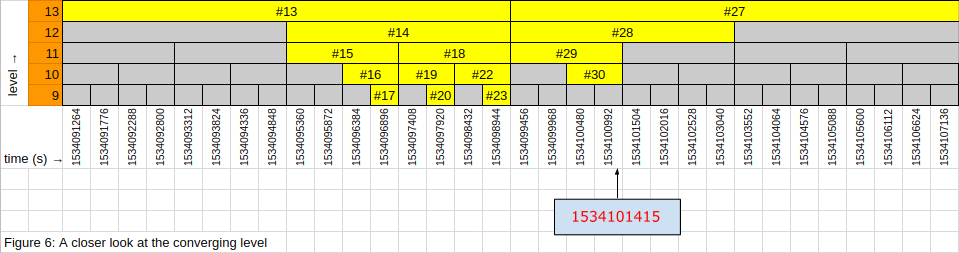
\includegraphics[width=\textwidth]{fig/feeds/03.png}
\caption[Updates of epoch-based feed in the epoch grid]{Updates of epoch-based feed in the epoch grid. Epochs occupied are marked in yellow. }
\label{fig:feeds-update}
\end{figure}

If the publisher keeps updating every 5 minutes ($300s$), we can expect the updates to stay around level 8-9 ($2^8 = 256s$, $2^9 = 512s$). The publisher can however, at any time vary this update frequency or just update randomly. This does not affect the algorithm.

\subsection{Parallel algorithm to look up the latest update \statusorange}\label{sec:feeds-lookup-algo}

This section gives a walkthrough about the steps of the algorithm that finds the latest update of a epoch-based feed  (see \ref{sec:epoch-based-feeds}).

\begin{figure}[htbp]
\centering
\begin{tabular}{c|c}
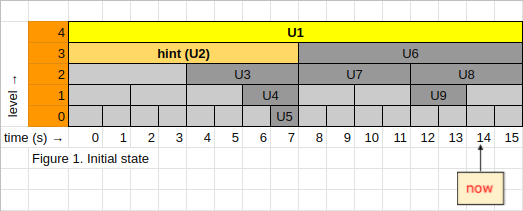
\includegraphics[width=.5\textwidth]{fig/feeds/0.png}&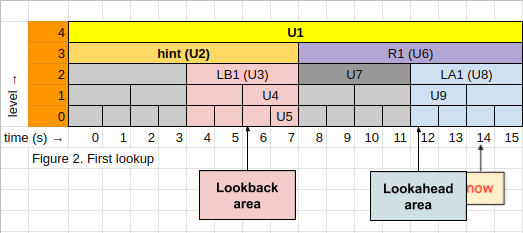
\includegraphics[width=.5\textwidth]{fig/feeds/1.png}\\
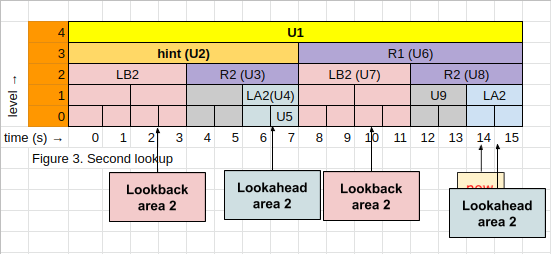
\includegraphics[width=.5\textwidth]{fig/feeds/2.png}&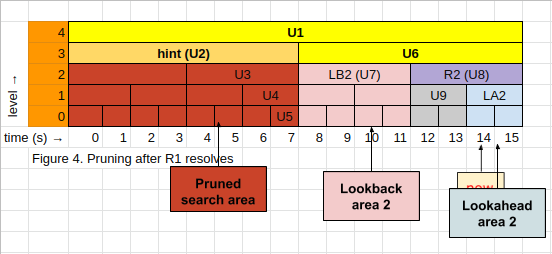
\includegraphics[width=.5\textwidth]{fig/feeds/3.png}\\
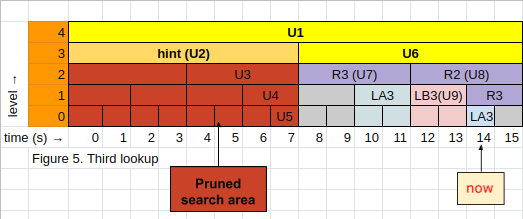
\includegraphics[width=.5\textwidth]{fig/feeds/4.png}&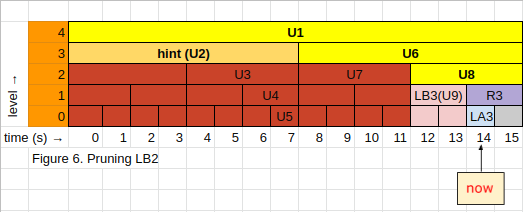
\includegraphics[width=.5\textwidth]{fig/feeds/5.png}\\
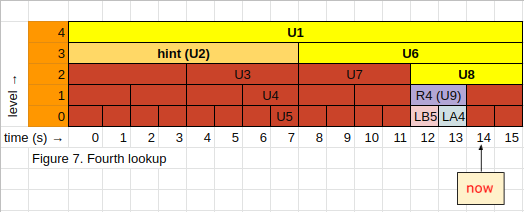
\includegraphics[width=.5\textwidth]{fig/feeds/6.png}&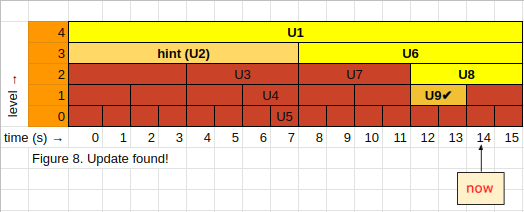
\includegraphics[width=.5\textwidth]{fig/feeds/7.png}
\end{tabular}
\caption[Latest update lookup algorithm for time based feeds]{Latest update lookup algorithm for time based feeds: steps. Known updates (U1) are marked in yellow. The hint is light orange (U2). Updates marked in grey (U3-U9) are unknown. $t=14$ indicates the current time, Step 1: lookahead (LA1) area (blue) and lookback (LB1) area (pink); }
\label{fig:feeds-lookup-1}
\end{figure}

The \gloss{lookahead area} indicates the area that will continue to be explored if R1 succeeds, while the \gloss{lookback area} highlights what will be continued to be explored if R1 fails to find an update at their location. After a short interval (configurable parameter \gloss{head start}) waiting for R1 to resolve, the algorithm sets out to explore both lookahead and lookback areas, headed by  $\langle  12, 2 \rangle$ and $\langle  4, 2 \rangle$ respectively. These two simultaneous lookups are labeled R2 in the figure below, and are active together with R1. Also, recursively, 4 more lookup areas (labeled LA2 and LB2) are defined that depend on the result of each instance of R2:
Once R1 resolves we can prune one area or the other. This is implemented by recursively cancelling a context, which aborts all chunk retrievals associated with it. The found update U9 can then be used as a hint for future lookups

In our example, R1 returns update U6, therefore our status is as below. Note that U6 is now marked as "known" in yellow, thus we're certain that the area in dark red, while it could contain other updates, **does not contain the latest one**, which is the one we care about:


Again, after a short head start, the algorithm proceeds to look up the lookback and lookahead headers $\langle  8, 2 \rangle$ and $\langle  14, 1 \rangle$, marked as active (purple), with the label R3 below. These come, recursively, with their own lookahead and lookback areas, labeled LA3 and LB3:

In our example, R2 finally resolves, finding update U8. This means we can cancel lookback area LB2 as we are now sure the last update can't be there:


To shorten up the example, if R3 resolved immediately with no update found ($\langle  14, 1 \rangle$ did not contain an update), that would cancel LA3 family of lookups, while LB3 continues (now marked as R4):


Although not drawn above, it is easy to see the pattern: LA4 and LB5 would then be scanned as R5 and R6 respectively, and in this case, fail, thus leaving $\langle  12, 1 \rangle$ (U9), as the found update:


.

This example is simplified -- with the current algorithm parameters, there can potentially be around 30 lookups taking place concurrently, exploring the search space for updates and pruning entire branches recursively once a better path is found. This can be configured by adjusting the lookup timeout and headstart times.

If the algorithm failed to find an update (i.e., if U3-U9 did not actually exist), then the hint in $\langle  0, 3 \rangle$ (U2) would be challenged for validity: In this situation if the hint actually contains an update, that is then returned the last update and we're done. If the hint, however, is proven false then the algorithm restarts without hint at that point.


\chapter{Implementers' guide}\label{sec:implementor-guide}

\section{Kademlia data structure \statusred}    
                        
\section{Local store \statusred}

\section{Concurrent hashing \statusred}



\chapter{About the project \statusred}\label{sec:about}
\section{History \statusred}
\section{Organisation \statusred}
\section{Community \statusred}
\section{Ecosystem \statusred}